\documentclass[a4paper, 12pt, ngerman, twoside, openright]{scrreprt}

% Rendering packages
\usepackage{amsmath}
\usepackage{amssymb}
\usepackage{graphicx}
\usepackage{color}
\usepackage{fancyvrb}

% Page dimensions
\usepackage[inner=3.5cm,outer=2.5cm,top=3.7cm,bottom=3.5cm]{geometry} % Settings for twoside documents.
\usepackage{parskip}

% Font styling
\usepackage[ngerman]{babel}
\usepackage[utf8]{inputenc}
\usepackage[T1]{fontenc}
\usepackage{lmodern}
\renewcommand\familydefault{\sfdefault}

% Tables
\usepackage{tabularx}
\usepackage{tabulary}
\usepackage{longtable, lscape}

% Headers
\usepackage{scrpage2}  % header and footer for KOMA-Script
\pagestyle{scrheadings}
\automark[section]{chapter}
\usepackage{marvosym} % für Euro-Zeichen

% Zitate
\usepackage[backend=bibtex, style=numeric, sorting=none]{biblatex}
\usepackage[babel,german=guillemets]{csquotes}
\bibliography{Bibliothek/Bibliothek}

\usepackage[hyperindex,breaklinks,colorlinks=true,linkcolor=black,urlcolor=blue,citecolor=black]{hyperref}

% Code Blöcke
\usepackage{listings}

% Listings konfigurieren.
\lstset{language=[Objective]C, 
        breakindent=40pt, 
        breaklines, 
        frame=lines,
        morekeywords={id, Class, SEL, IMP, BOOL, nil, Nil, NO, YES,
                  oneway, in, out, inout, bycopy, byref,
                  self, super, _cmd,
                  @required, @optional,
                  @try, @throw, @catch, @finally,
                  @synchronized, @property, @synthesize, @dynamic},
        basicstyle=\ttfamily\scriptsize,
        literate=
            {Ö}{{\"O}}1
            {Ä}{{\"A}}1
            {Ü}{{\"U}}1
            {ß}{{\ss}}2
            {ü}{{\"u}}1
            {ä}{{\"a}}1
            {ö}{{\"o}}1}
        
\definecolor{dkgreen}{rgb}{0,0.6,0}
\definecolor{gray}{rgb}{0.5,0.5,0.5}
\definecolor{mauve}{rgb}{0.58,0,0.82}
\definecolor{orange}{rgb}{1,0.35,0.2}
\definecolor{lightblue}{rgb}{0.53,0.81,0.98}        

\lstset{frame=tb,
	language=Java,
	aboveskip=3mm,
	belowskip=3mm,
	showstringspaces=false,
	columns=flexible,
	basicstyle={\small\ttfamily},
	numbers=none,
	numberstyle=\tiny\color{gray},
	keywordstyle=\color{blue},
	commentstyle=\color{dkgreen},
	stringstyle=\color{mauve},
	breaklines=true,
	breakatwhitespace=true,
	tabsize=3
}

\lstdefinelanguage{drools}{frame=tb,
	morekeywords={rule, rule, when,then, end, end}
	aboveskip=3mm,
	belowskip=3mm,
	showstringspaces=false,
	columns=flexible,
	basicstyle={\small\ttfamily},
	numbers=none,
	numberstyle=\tiny\color{lightblue},
	keywordstyle=\color{orange},
	breaklines=true,
	breakatwhitespace=true,
	tabsize=4}

%NEW COMMANDS
\newcommand\tab[1][1cm]{\hspace*{#1}}

%Verfickte Glossare
\usepackage[nonumberlist,acronym,toc]{glossaries}
\makeglossaries
\newacronym[]{BSP}{BSP}{Beispiel Abkürzung}

\newglossaryentry{Beispiel Glossary Entry}
{
  name=Constrain-Satisfaction-Problem,
  description={Ein Constraint-Satisfaction-Problem besteht aus einer Menge von Variablen, ihren Wertebereichen und den Bedingungen, die Verknüpfungen zwischen den Variablen herstellen und dadurch festlegen, welche Kombinationen von Werten der Variablen zulässig sind}
}



\begin{document}



% Titelseite einfügen.
%Titelseite
% Seitennummer aus
\thispagestyle{empty}

\begin{titlepage}

\vspace{3cm}

\begin{center}
	%\includegraphics[scale=0.8]{Titelseite/Logo.pdf}  
\end{center}

\vspace{2.5cm}

\begin{center}
  \Large FAKULTÄT FÜR INFORMATIK
\end{center}

\vspace{1cm}
\begin{center}
	\Huge
	\textbf{Master Arbeit}\\
\end{center}

\vspace{1cm}

\begin{center}
	\Large
	\textbf{Digitalisierung im Handwerk}
\end{center}

\vspace{1.5cm}

\begin{center}
	\Large
	Fabian Kloos
\end{center}

\vspace{3.5cm}

\begin{center}
    \large
	\textbf{Betreuer}
\end{center}

\vspace{0.3cm}

\begin{center}
    \large
    bla bla bla Betreuer
\end{center}

\newpage
\thispagestyle{empty}
\mbox{}
\end{titlepage}


% Counter zurücksetzen. Römische Ziffern einstellen.
\pagenumbering{Roman}
\setcounter{page}{1}

% Selbständigkeitserklärung einfügen.
\chapter*{Selbstständigkeitserklärung}
Hiermit erkläre ich, dass ich die Arbeit selbständig verfasst, noch nicht anderweitig für Prüfungszwecke vorgelegt, keine anderen als die angegebenen Quellen oder Hilfsmittel benützt, sowie wörtliche und sinngemäße Zitate als solche gekennzeichnet habe.

\vspace{2cm}

\begin{tabular}{@{}ll@{}}
......................... &  .................................................. \\
Datum                     &  Fabian Kloos
\end{tabular}


% Abstract einfügen.
\chapter*{Abstract}

Die vorliegende Masterarbeit analysiert den aktuellen Stand der Digitalisierung im Handwerk, sowie kleinen und mittleren Unternehmen und findet auf dieser Grundlage Bereiche, die Unterstützung benötigen. Darauf basierend wird ein Augmented Reality Applikation für Fliesenleger entwickelt und ihr Mehrwert für Handwerker bestimmt. Durch eine Fokusgruppe und eine Ethnographie werden Daten zu Problemen von Handwerkern erhoben und Ansätze für ein Unterstützungswerkzeug gefunden. Daraus wird eine Microsoft HoloLens Applikation für Fliesenleger mithilfe von gestaltungsorientierter Forschung implementiert, welche anschließend mit Handwerkern durch einen Fragebogen und ein Interview evaluiert wird. Die Ergebnisse bestätigen die Annahme, dass Augmented Reality als Visualisierungswerkzeug für Kundengespräche und zur Unterstützung bei der Arbeit für Handwerker interessant ist. Schlussfolgernd lässt sich sagen, dass Datenbrillen für Augmented Reality noch nicht genügend ausgereift sind, in Zukunft jedoch für Handwerker interessant sein können.

The present master thesis analyses the current state of digitisation in crafts, as well as small and medium-sized enterprises, and on this basis finds areas that require support. Based on this, an Augmented Reality application for tilers will be developed and its added value for craftsmen will be determined. Through a focus group and an ethnography data on problems of craftsmen will be collected and approaches for a support tool will be found. From this, a Microsoft HoloLens application for tilers will be implemented using design science, which will then be evaluated with craftsmen through a questionnaire and an interview. The results confirm the assumption that Augmented Reality is interesting for craftsmen as a visualization tool, for advising customers and to support their work. In conclusion, it can be said that head mounted displays for augmented reality are not yet sufficiently mature, but may be interesting for craftsmen in the future.

% Inhaltsverzeichnis generieren.
\tableofcontents

% Neue Seite. Counter zurücksetzen. Arabische Ziffern einstellen.
\cleardoublepage
\pagenumbering{arabic}
\setcounter{page}{1}

% Kapitel einfügen.
\chapter{Methoden}

Dieses Kapitel behandelt die in dieser Arbeit angewandten Methoden zur Erhebung der Daten und Erarbeitung der Lösung zu einem gefundenen Problem. Es soll die Vorgehensweise theoretisch beschreiben und untermauern.

\section{Fokusgruppe}
\label{sec:fokus}

Bei einer Fokusgruppe handelt es sich um ein moderiertes Diskursverfahren, bei dem ein Meinungsbild durch die Interaktion einer ausgewählten Gruppe erzeugt wird und somit Daten über ein festgelegtes Thema erhoben werden. Man kann es als Kombination aus fokussiertem Interview und Gruppendiskussion sehen. Als Instrument zur Datenerhebung in den Sozialwissenschaften hat es sich in den 60er und 70er Jahren etabliert. Es wird für folgende Felder verwendet \cite{schulz_quick_2012}:

\begin{itemize}
	\item Testverfahren
	\item Analyse an Meinungsvielfalt
	\item Instrument zur Akzeptanzanalyse
	\item Instrument zur Konfliktschlichtung
	\item Evaluierung bestimmter Maßnahmen
	\item Technikvorausschau
	\item Analyse heikler Aspekte aus dem Gesundheitsbereich
\end{itemize}

Normalerweise bestehen die Gruppen aus sechs bis zwölf Personen und einem Moderator. Die Gruppengröße kann jedoch auch erhöht werden, um eine bessere Repräsentanz zu erhalten. Alle Teilnehmer können je nach Ziel der Fokusgruppe zufällig oder nach Kriterien, wie Geschlecht, Lebensstil oder Beruf gewählt werden. Bestenfalls kennen sich die Teilnehmer untereinander nicht. \\
Der Moderator hat die Aufgabe den Dialog zwischen den Diskutierenden am laufen zu halten. Die Diskussion soll ein lebendiges Gespräch sein, welches von den Teilnehmern getragen und durch den Moderator, der sich an einem Leitfaden als Gedächtnisstütze orientiert, gelenkt wird. Er achtet auch darauf, dass Personen nicht durcheinander reden. Bohnsack und Schäffer legen vier Vorgehensweisen eines guten Moderators fest \cite{bohnsack_gruppendiskussionsverfahren_2001}:

\begin{itemize}
	\item Unterlassung inhaltlicher Stellungnahmen
	\item Ansprechen der gesamten Gruppe bei Interventionen
	\item Fragen nicht an Einzelne, sondern an das Kollektiv richten
	\item Vermeidung der Individualkommunikation von einzelnen Teilnehmern mit dem Moderator
\end{itemize}

Der Ablauf einer Fokusgruppe lässt sich in drei Phasen unterteilen \cite{schulz_quick_2012}. Die \textit{erste Phase} dient der inhaltlichen und organisatorischen Vorbereitung der Fokusgruppe. Der Moderator erstellt den Leitfaden und bestimmt und rekrutiert die Gruppe an Personen. Die Fokusgruppe leitet er dann mit einem Film, Bild, einer Homepage oder einem Vortrag ein, um den Teilnehmern das Thema näher zu bringen.\\
Die Diskussion stellt die \textit{zweite Phase} und die umfangreichste dar. Die Aufgabe des Moderators ist es dabei, das Gespräch anzuregen und dafür zu sorgen, dass jeder Teilnehmer einbezogen wird und aktiv an der Diskussion teilnimmt. Es ist für den Moderator von Vorteil einen Assistenten zu haben, der sich um kleinere Aufgaben und das Protokollieren der Erkenntnisse kümmert. Dies sollte schriftlich festgehalten werden und kann durch Audioaufzeichnungen und/oder Videoaufzeichnungen komplementiert werden. Videos sind dabei mit Vorsicht zu nutzen, da diese das Teilnahmeverhalten der Teilnehmer negativ beeinflussen können. \\
Das Meinungsspektrum der Gruppe ist dabei das interessante Ergebnis. In der \textit{dritten Phase}, der Datenanalyse und Interpretation der Ergebnisse müssen alle Aufzeichnungen, also schriftliche, Video- und Audioaufnahmen gemeinsam ausgewertet werden. So erhält man eine Sammlung an Meinungen der gesamten Gruppe, welche teilweise repräsentativ für ein bestimmtes Feld sind.

\section{Ethnographie: Teilnehmende Beobachtung}

\textit{``Will man etwas über andere Menschen herausfinden, \\
	geht man einfach zu ihnen hin, bleibt eine Weile, \\ 
	macht das mit, was diese Menschen dort normalerweise treiben, \\ 
	und lernt sie so durch eigene Erfahrung besser kennen.`` - Götz Bachmann} \cite{kuhl_handbuch_2009}

\subsection{Zusammensetzung der Methode}

Es sollen nun Ansatzpunkte gefunden werden, um die Theorie "Handwerker können durch den Einsatz von Technologie unterstützt werden und Zeit sparen" zu stärken. In der Ethnographie unterscheidet man dabei drei Varianten \cite{spittler_teilnehmende_2001}:

\begin{itemize}
	\item \textbf{Sammelzentriert:} Ethnographie unter der Prämisse, man muss und kann alle Informationen zu einem Gebiet sammeln.
	\item \textbf{Theoriezentriert:} Beobachtetes und Fakten werden "im Lichte einer Theorie" ausgewählt und geordnet. Hierzu zählt unter anderem die teilnehmende Beobachtung.
	\item \textbf{Problemzentriert:} Die Ethnographie stellt ein komplexes Problemfeld vor. Der Fokus liegt dabei nicht auf den Theorien des Forschers.
\end{itemize}

Diese Ethnographie fällt unter zweitere Kategorie, da die Aufzeichnungen genutzt werden, um oben genannte Theorie zu untersuchen. 

Im klassischen Sinne werden Sachverhalte durch Fragebögen und systematische Interviews beleuchtet. Mit diesen Methoden können zwar in kurzer Zeit viele Informationen erhoben werden, jedoch werden sie häufig als extrem künstlich kritisiert. Diese statische Atmosphäre kann dazu führen, dass kein gutes Gespräch zustande kommt und der Handwerker nur genau auf die Fragen antwortet und Informationen zurückbehält. Der Fakt, dass berufliches Wissen oft als Geheimnis angesehen und nur spärlich und selektiv weitergegeben wird, spielt hier noch negativ mit ein \cite{spittler_teilnehmende_2001}. Deshalb sollten Fragebogen und Interview für diese Forschung noch komplementiert werden.

Ein Blick fängt oft mehr ein als Worte. Deshalb wird zum Erheben der Informationen noch die Beobachtung der Arbeit eines Handwerkers hinzugefügt. Laut Spittler \cite{spittler_teilnehmende_2001} gibt es drei Prämissen, die eine Beobachtung, zusätzlich zu einem Interview befürworten:

\begin{enumerate}
	\item "Forschungspragmatisch besitzt die Beobachtung in manchen Situationen einen Vorteil gegenüber der Befragung."
	\item "Die sprachliche Erfassung stößt wegen Geheimhaltung, Schweigen und Verschweigen auf Schwierigkeiten."
	\item "Handlungen sind sprachlich gar nicht oder nur unter großen Schwierigkeiten erfassbar. (tacit knowledge)"
\end{enumerate}

Um die Arbeit eines Handwerkers besser zu verstehen, reicht es nicht sich diese nur von ihm Beschreiben zu lassen. Bei der Ausübung seines Handwerks kann er keine Schritte "verschweigen" und der Forscher kann diese direkt analysieren. Indem er sein Notizheft beiseite legt und selbst mitarbeitet, kann er sich ein genaues Bild des Handwerks machen und so auch kleine Ansatzpunkte zum bekräftigen seiner Theorie finden \cite{malinowski_argonauts_1922}. Deshalb wurde die Teilnehmende Beobachtung als Methode der Ethnographie gewählt.

\subsection{Beschreibung der Methode}

Feldforschung ist eine der ältesten und am weitesten verbreiteten Techniken zur Datenerhebung in einem unbekannten Forschungsgebiet. Die Forschungspraxis hängt dabei in hohem Maße von der \textit{Persönlichkeit der Forschers}, der \textit{Beschaffenheit des Feldes} und der \textit{Interaktion des Forschers mit dem Feld} ab. Das bedeutet die Forschung lässt sich schlecht genau durchplanen und der Forscher kann sie nur begrenzt kontrollieren. Einige Ethnologen argumentieren, dass gerade das den Reiz der Methode ausmacht \cite{rottenburg_feldforschung_nodate}. Andere bezeichnen die teilnehmende Beobachtung deshalb als "methodenfeindlich" \cite{kuhl_handbuch_2009}. Daraus geht hervor, dass es keinen besten Weg gibt diese Methode durchzuführen, nur Anregungen und Tipps.

Zur Datenerhebung sind die Punkte \textit{Forschungsanfang}, \textit{Rollenzuweisung}, \textit{Beobachtungsdauer}, \textit{wo und wie beobachtet wird}, sowie das \textit{Aufschreiben der Erlebnisse} zu beachten \cite{kuhl_handbuch_2009}. Diese werden im Folgenden erläutert. \\
Der erste Tag im Feld ist laut Bachmann einer der anstrengendsten. Nicht nur Beobachten und die ersten Eindrücke verarbeiten, muss der Forscher an diesem Tag, es kommen auch einige soziale Aufgaben auf ihn zu. Er muss die neuen Kollegen in seinem Forschungsumfeld kennenlernen, sowie überlegen, wie er sich diesen gegenüber gibt. Am besten sollte er sich neutral präsentieren und sich nicht verstellen, um ein nettes Verhältnis den zu Erforschenden gegenüber aufzubauen. Das erzeugt gegenseitiges Vertrauen. Trotzdem sind seine Eindrücke in den ersten Tagen dadurch getrübt. \\
Meist schlüpft der Forscher hierbei in die Rolle des Praktikanten, der nicht viel kann, viel nachfragt und viel herumkommt. Andere Ansätze erwähnen auch die Rollen Auszubildender, Lehrling oder Trainee, welche jedoch weniger flexibel sind und dem Forscher eine geringere Bewegungsfreiheit bieten. \\
Im klassischen Sinne wurde eine Ethnographie über einen langen Zeitraum von ca. einem Jahr durchgeführt, was beispielsweise bei der Untersuchung des Arbeitsalltags auf einem Bauernhof Sinn ergab, jedoch in der modernen Forschung kaum mehr tragbar ist. Nun ist eine Dauer von zwei bis sechs Monaten üblich. Auch Zeiträume von einem Tag bis zu ein oder zwei Wochen können schon wertvolle Ergebnisse liefern, wecken jedoch Skepsis bei einigen Ethnologen. \\
Während der Arbeit beobachtet der Forscher kleine Details, die eventuell bei Gesprächen übergangen, oder nicht ausreichend wörtlich wiedergegeben werden können. Pausen, sowie die Zeit vor und nach der Arbeit, also Daten aus informellen Situationen, werden von einigen Forschern als sehr wichtig angesehen, da sie dem Forscher die Möglichkeit bieten sich mit den Erforschten auszutauschen und neue Kontakte zu knüpfen, über die er wieder neue Erkenntnisse oder Einblicke erlangen kann. Wie er an die besten Daten bekommt ist jedoch immer forschungsabhängig. Organisationsforscher legen dabei mehr Wert auf die Beobachtung der Arbeit. Graaf und Rottenburg \cite{rottenburg_feldforschung_nodate} sprechen hier von "dabeistehender Beobachtung", welche der Forscher ausführt, da er selbst wahrscheinlich nicht die Fähigkeiten besitzt, um die Tätigkeit selbst auszuführen. Er konzentriert sich also auf das Beobachten, Fragen stellen und führt eventuell Hilfstätigkeiten aus. Um spezielle Informationen zu erlangen, kann sich der Ethnologe auf \textit{Konflikte} konzentrieren, welche viel über die Organisation und die involvierten Personen aussagen. Ein anderer Ansatz ist, in "Anbedacht des Unbedeutenden" sein gesamtes Augenmerk auf eine kleine Bagatelle zu richten. Außerdem kann der Forscher einmalige, kleine Situationen herausgreifen und diese anhand des Kontexts und seines erworbenen Wissens analysieren. \\
Um das Wissen festzuhalten, macht sich der Ethnologe am besten direkt nach einem Sachverhalt Notizen für später, als Erinnerungsstütze. Das hilft ihm beim zweiten Schritt, dem Ausformulieren in einem Forschungstagebuch. Dabei kann er entweder das erlebte sachlich und in der Ausführung präzise beschreiben, oder bereits beim Ausformulieren seine Interpretationen einfließen lassen. Auch das ist wieder abhängig von der betriebenen Forschung. Er sollte sich von Anfang an einen Zitierstil zum kennzeichnen von verschiedenen Zitaten in unterschiedlichen Kontexten aneignen und konsequent durchziehen. Zusätzlich zum Forschungstagebuch kann der Ethnologe ein Tagebuch für \textit{persönliche Gefühle und Erfahrungen}, \textit{Ideen und theoretische Erwägungen} und/oder einen \textit{Forschungskalender}, in den er seine nächsten Schritte einträgt, führen. Oft reicht die Zeit nach Feierabend nicht aus, um alle Erlebnisse nachzutragen, weshalb es auch sinnvoll sein kann sich unter Tags Zeit und einen Platz zum Arbeiten zu schaffen. 

Mit dieser Methode lässt sich ein Beruf analysieren, wobei man nicht alle Einzelheiten festhalten kann. Dadurch ist es dem Forscher möglich Ansatzpunkte für weitere Forschung oder Verbesserungen zu finden.

\section{Gestaltungsorientierte Forschung: Implementieren eines Prototypen}
\label{sec:gestForsch}

Mit den Methoden Fokusgruppe und Ethnographie wird ein bestehendes Problem genauer beleuchtet und dabei herausgearbeitet, ob die Lösung dieses Problems wünschenswert ist. Auf Basis des erörterten Umstands soll dann eine Lösung gefunden werden, die dem Forscher und allen beteiligten Parteien genügt. Dabei stellt sich die Frage, wie man das Problem adressiert. Für problembasierte Forschung ist der Weg zu einer Lösung nicht geradlinig, weshalb ein flexibler Ansatz genutzt werden soll, wofür sich laut Hevner et al. \cite{hevner_design_nodate} die Methode \textit{Gestaltungsorientierte Forschung} anbietet. Dabei wird von einem Problem augegangen und über einen inkrementellen, iterativen Prozess eine Lösung erarbeitet. Hevner identifiziert dazu fünf charakteristische Faktoren von Problemen, die mit gestaltungsorientierter Forschung angegangen werden \cite{hevner_design_nodate}:

\begin{enumerate}
	\item ``Environmental factors such as requirements and constraints are poorly defined"
	\item ``An inherent complexity in the problem and possible solutions"
	\item ``A flexibility and potential for change of possible solutions"
	\item ``A solution at least partially dependent on human creativity"
	\item ``A solution at least partially dependent on collaborative effort"
\end{enumerate}

Das Erfüllen dieser Kriterien qualifiziert ein Problem für gestaltungsorientierte Forschung. Basierend auf den Arbeiten von Hevner und anderen renommierten Wissenschaftlern entwickelte Pfeffers ein \textit{6-Phasen Modell} zur Durchführung einer solchen Forschung \cite{j._ellis_guide_2010}. Dabei werden die Phasen \textit{Problemidentifikation und Motivation} zur Begründung der Forschung, \textit{Ziel der Lösung}, \textit{Gestaltung und Entwicklung}, sowie \textit{Demonstration des Artefakts}, \textit{Evaluation} der Tests und \textit{Kommunikation der Ergebnisse} durchlaufen \cite{peffers_design_2007}. 

\begin{figure}[h]
	\begin{center}
		\noindent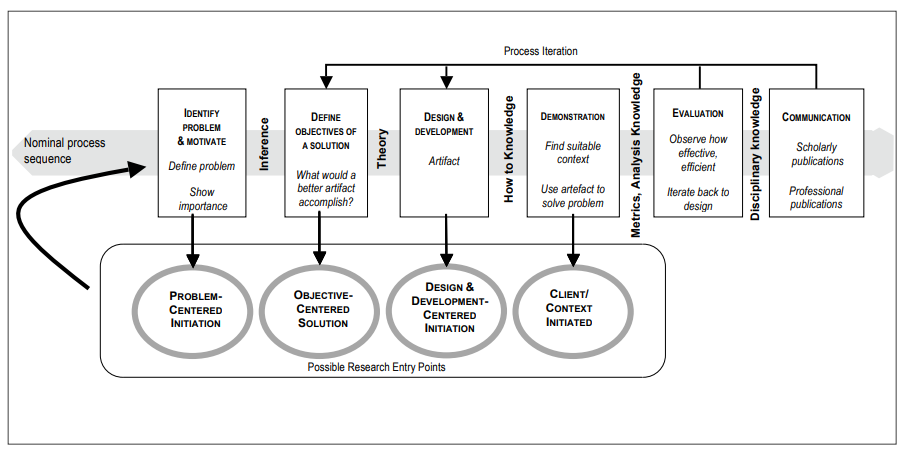
\includegraphics[width=\linewidth,height=\textheight,keepaspectratio]{Resources/DS_Peffers.png}
		\caption{Peffers et al.: Gestaltungsorientierte Forschung \cite{peffers_design_2007}}
	\end{center}
\end{figure}

Diese sechs Phasen können sequentiell von der ersten bis zur letzten durchgearbeitet werden, aber nicht zwangsläufig. Ein Forscher kann auch an einer für ihn passend erscheinenden Phase beginnen und von dort aus weiterarbeiten. Problemzentrierte Forschung beginnt in Phase 1, \textit{Problemidentifikation und Motivation}. Dieser Ansatz wird häufig gewählt, wenn auf früherer Forschung aufgebaut oder von der Beobachtung eines Problems begonnen wird. Zielorientierte Forschung hingegen startet meistens in Phase 2, \textit{Ziel der Lösung}. Dies wird oft durch einen Anstoß aus der Industrie angetrieben. Gestaltungsorientierte Ansätze beginnen mit Phase 3, \textit{Gestaltung und Entwicklung}. Dabei gehen die Forscher meist von einem unfertigen, nicht komplett durchdachten Artefakt aus früherer Forschung oder Projekten aus. Eventuell stammt das Artefakt sogar aus einer anderen Forschungsdomäne und wurde zur Lösung eines anderen Problems erstellt. Mit Phase 4, \textit{Demonstration des Artefakts} beginnt die kunden- oder kontextbasierte Forschung. Dabei entstand die Idee beim Beobachten einer praktischen Lösung, welche funktioniert. Die Forscher arbeiten dabei rückwärts und versuchen so die bestehende Lösung zu verbessern. Dieser Ansatz kann aus einer Consultingerfahrung hervorgehen.

In dieser Arbeit wird mit Phase 1 begonnen, da das Problem anfangs durch die Ethnographie identifiziert wurde. Im Folgenden wird die Methode von Peffers genauer beschrieben \cite{peffers_design_2007}.

\subsection{Problemidentifikation und Motivation}

Peffers diskutiert Ansätze verschiedener Wissenschaftler zu Problemidentifikation und wie man Ideen findet, welche umsetzenswert sind. Der Ansatz, welcher von Pfeffers aufgegriffen wird, von Archer \cite{archer_systematic_1965} und Eekels \cite{eekels_methodological_1991} bezieht sich auf angewandte Probleme, also welche die bei einer Tätigkeit auffallen, auftreten und behindern. \\
In diesem Abschnitt muss die Suche nach einer Lösung für ein Problem begründet werden. Der zu betrachtende Umstand wird dafür genau dargelegt und definiert. Das Problem wird in kleine Teile gespalten und genau beleuchtet. Durch eingehende Betrachtung kleiner Teilbereiche kann die Komplexität des Problems in der Lösung abgebildet werden. Nur aus einer ausreichenden Problembeschreibung lässt sich ein fundiertes Artefakt erzeugen. 

Aus der Motivation ergeben sich zwei Vorteile für den Forscher: \\
Das Problem zu identifizieren und so die Suche nach einer Lösung zu begründen motiviert den Forscher, sowie die Leser seiner Arbeit bei der Suche und der Akzeptanz der Ergebnisse. \\
Zusätzlich hilft es Lesern seine Schlussfolgerungen nachzuvollziehen. \\
Um diesen Schritt durchzuführen stehen das Wissen über den aktuellen Stand des Problems, sowie die Wichtigkeit der Lösung als Ressourcen zur Verfügung. Daraus lassen sich die Anforderungen an eine Lösung zusammenstellen \cite{peffers_design_2007}.

\subsection{Ziel der Lösung}

Auch wenn das Problem gut spezifiziert ist, lässt es sich oft nicht direkt in Ziele übersetzen. Diese lassen sich besser über einen inkrementellen Prozess bestimmen, als direkt festlegen. Damit sollen die performance Ziele der Lösung herausgearbeitet werden. 

Grundlegend leitet man die Ziele von der Problemdefinition, sowie dem Wissen was möglich und machbar ist ab. Dabei kann das Ziel quantitativ sein, also beispielsweise Umstände darlegen, für welche die angestrebte Lösung besser ist als eine existierende. Oder es handelt sich um ein qualitatives Ziel, bei dem ein Artefakt Lösungen oder Hilfe für Probleme bereitstellt, welche über das ursprüngliche Problem hinausgehen. Besonders wichtig ist dabei, dass alle Ziele logisch aus der Problemspezifikation herleitbar sind. Als Ressource zur Herleitung der Ziele sollte der aktuelle Stand des Problems, als auch bereits verfügbarer Lösungen (falls existent), vorhanden sein und deren Zweckmäßigkeit überprüft werden.

\subsection{Gestaltung und Entwicklung}

Aus den gefundenen Problemen und Zielen wird nun ein Artefakt entwickelt. Für Peffers Gestaltungsorientierte Forschung kann man dabei nach dem Prinzip "early prototyping" vorgehen, da es sich um einen inkrementellen Prozess handelt. Alle Wissenschaftler, welche Peffers untersuchte legten den Fokus auf diese Phase.

Es wird dabei ein Artefakt erzeugt. Artefakte sind für Peffers Konstrukte, Modelle, Methoden, Instantiierungen oder "new properties of technical, social, and/or informational resources" \cite{jarvinen_action_2007}. Generell ist dabei jedes Forschungsartefakt ein Objekt, welches durch Zuhilfenahme von wissenschaftlichen Beiträgen entstanden ist. Dies beinhaltet die Funktion und die Architektur des Artefakts festzulegen und daraus dann das Artefakt zu kreieren. Dabei soll der Wissenschaftler theoretisches Wissen als Ressource nutzen, welches in der Lösung zum tragen kommen soll.

\subsection{Demonstration des Artefakts}

Um die Funktionstauglichkeit des Artefakts zu testen wird es vorgezeigt. Dabei kann entweder ein Test stattfinden, um zu zeigen, dass die Idee funktioniert, oder mehrere Tests, um eine genauere Evaluation durchzuführen.

Das Artefakt wird dabei so vorgeführt, damit deutlich wird, dass es eins oder mehr der anfangs definierten Probleme lösen kann. Dazu zählt die Verwendung des Artefakts in Experimenten, Simulationen, Case Studies, Beweisen oder anderen geeigneten Aktivitäten. Als Ressource zum Durchführen der Demonstrationsphase gilt das Wissen, wie man das Artefakt einsetzen muss, um ein Problem zu lösen.

\subsection{Evaluation}

Das Artefakt wurde untersucht und nun müssen die Informationen verwertet werden. Dazu ist wichtig, dass vor der Demonstration Werte festgelegt werden, welche dabei erfasst werden. Der Wissenschaftler muss genau beobachten und messen, wie gut das Artefakt die Lösung des Problems unterstützt. Dazu vergleicht er die Ziele der Lösung mit den tatsächlich beobachteten Ergebnissen der Demonstration des Artefakts. Um dies erfolgversprechend durchzuführen, wird ein Wissen über relevante Metriken und Analysetechniken verlangt.

Der Charakter der Forschung entscheidet dabei, welche Form der Evaluation durchgeführt wird. Dabei werden Methoden verwendet, wie beispielsweise das Vergleichen der Artefaktfunktionalität mit den Zielen der Lösung aus Phase 2, quantitative Leistungsmesswerte, wie hergestellte Güter oder erwirtschaftetes Kapital, Ergebnisse von Zufriedenheitsumfragen, Kundenfeedback, Simulationen, oder quantifizierbare Messwerte der Systemperformanz, wie Reaktionszeit oder Verfügbarkeit des Systems. Die Evaluation kann alle möglichen geeigneten empirischen Daten oder logische Beweise enthalten.

Am Ende dieser Phase kann der Forscher entscheiden ob er wieder zu Phase 3 zurückgeht und die gewonnenen Erkenntnisse nutzt um ein neues, besseres Artefakt zu entwickeln, oder ob er in die letzte Phase der Methode fortschreitet und die weitere Entwicklung zukünftigen Projekten überlässt. Dabei gibt die Art der Forschung an, welche Methode sinnvoller ist.

\subsection{Kommunikation der Ergebnisse}

Die gewonnenen Erkenntnisse müssen nun entsprechend Kommuniziert werden, um sie zu verbreiten. Dies sollte das Problem und seine Wichtigkeit, das Artefakt und seine Nützlichkeit und Neuartigkeit, die Einzelheiten des Designs und seine Effektivität enthalten. Die Publikation sollte an andere Wissenschaftler oder relevante Gruppen, wie zum Beispiel praktizierende Personen aus dem entsprechenden Bereich gerichtet sein. 

In wissenschaftlichen Publikationen kann die Struktur dieser Methode genutzt werden, um die Ausarbeitung zu strukturieren, wie beispielsweise empirische Forschung durch den empirischen Prozess (Problemdefinition, Literaturrecherche, Aufstellen der Hypothesen, Datensammlung, Analyse, Ergebnis und Fazit) strukturiert wird. Die Kommunikation der Ergebnisse erfordert Wissen darüber, wie Arbeiten in der entsprechenden Disziplin verfasst werden. 

\section{Designen des Fragebogens}

Diese Arbeit zielt darauf ab, einen theoretischen, sowie einen praktischen Beitrag abzuleiten. Dazu wurden Anmerkungen der Testpersonen während und nach den Probandentests notiert. Diese Informationen können dazu genutzt werden, Ideen zu sammeln und die Applikation zu verbessern, allerdings lassen sie sich nicht gut vergleichen. Sie stellen den praktischen Beitrag dar. Für den theoretischen Teil benötigt man vergleichbare Werte und Größen. Dazu wurde ein Evaluationsbogen konzipiert, der folgende Fragen beantworten soll:

\begin{itemize}
	\item Wie ist der Bezug des Handwerkers zu technischen Geräten?
	\item Wie komplex ist der Umgang mit dem System?
	\item Kann der Handwerker sich vorstellen die Technologie in Zukunft zu nutzen?
\end{itemize}

Ersteres soll Helfen abzuschätzen, wie sehr die technische Versiertheit des Handwerkers sich auf die Akzeptanz bzw. das Interesse an der Applikation auswirkt. \\
Die Nutzung eines neuen Systems, in diesem Fall einer AR Anwendung, stellt für die Handwerker aus unternehmerischer Sicht eine Risiko dar. Deshalb ist es essentiell bestimmen zu können, ob die Anwendung von den Nutzern akzeptiert und genutzt werden wird. Die beiden weiteren Fragen sollen Aufschluss darüber geben, wie die Einstellung der Fachkräfte zu dieser neuen Technologie ist. Um diese Fragen zu beantworten, werden psychologisch und wirtschaftlich evaluierte Modelle verwendet. 

Um die Gebrauchstauglichkeit der Applikation zu testen, wird das \textbf{SUS} (System Usability Scale) \cite{brooke_sus_nodate} Modell verwendet. Es gibt Aufschluss darüber, wie einfach oder umständlich die Bedienung für den Handwerker war. \\
Ein System wird nicht genutzt, wenn der Nutzer die Interaktion damit als zu Anstrengend empfindet. Um herauszufinden, als wie fordernd der Handwerker die Nutzung der Applikation empfindet, wird das Modell \textbf{NASA-TLX} verwendet. \\
Zusätzlich werden noch \textbf{TAM} und \textbf{TAM2} angewandt. Diese Abkürzungen stehen für Technology Acceptance Model. Sie wurden entwickelt, um vorherzusagen, wie wahrscheinlich ein Anwender eine Technologie nutzen wird. \\
Im folgenden werden die Modelle erklärt.

\subsection{SUS}

Bei der \textbf{System Usability Scale} handelt es sich um einen einfachen, aus zehn Punkten bestehenden Fragebogen zur subjektiven Einschätzung der Gebrauchstauglichkeit eines Systems. Es ist eine \textbf{Likert Skala}, auf welcher die Zustimmung oder Ablehnung durch sieben Punkte angegeben werden kann. Sie hilft Aufschluss darauf zu geben, ob ein System benutzt werden wird, oder nicht. \\
Nach ISO 9241-11 sollte die Messung der Gebrauchstauglichkeit folgende Aspekte abdecken \cite{brooke_sus_nodate}:

\begin{itemize}
	\item \textit{Effektivität:} Die Fähigkeit des Nutzers gestellte Aufgaben mit Hilfe des Systems zu erledigen und die Qualität der Resultate.
	\item \textit{Effizienz:} Die Menge der konsumierten Ressourcen, nötig zur Erledigung der Aufgabe.
	\item \textit{Befriedigung:} Die subjektiven Reaktionen des Nutzers auf die Verwendung des Systems.
\end{itemize}

Diese Größen zieht auch der industrielle Nutzer in Betracht, wenn er über die Implementierung einer neuen Technologie in seinem Arbeitsalltag nachdenkt. Aus unternehmerischer Sicht ist es jedoch oft nicht rentabel, eine komplette Kontextanalyse durchzuführen. SUS, mit seinen zehn Fragen, liefert eine genügende Einschätzung der Abdeckung dieser Größen.

Zur Erstellung des Fragebogens wurde ein Katalog von 50 Fragen durch John Brooke und sein Team analysiert. Dabei haben sie die zehn Fragen herausgearbeitet, welche die stärksten zustimmenden bzw. ablehnenden Reaktionen bei Probanden hervorgerufen haben. Durch die erhaltenen subjektiven Antworten auf diese Fragen lässt sich abschätzen, wie viel Training und Unterstützung neue Nutzer des Systems brauchen werden, um dieses erfolgreich zu benutzen, und wie komplex es den Anwendern erscheint.

Laut John Brooke \cite{brooke_sus_nodate} sollen die Probanden den Fragebogen ausfüllen, nachdem sie das System getestet haben und bevor eine anschließende Diskussion beginnt. Dabei sollen diese ankreuzen, was ihnen ihr Gefühl nach dem Lesen der Frage sagt und nicht lang über diese nachdenken. Alle Fragen müssen dabei beantwortet werden. Sollte ein Proband auf eine Frage keine Antwort geben wollen oder können, wird das neutrale Ergebnis der Frage angekreuzt. \\
Einzelne Antworten auf Fragen sind alleine nicht aussagekräftig. Die gesamte Auswertung aller Antworten gibt jedoch einen Wert zwischen 0 und 100, welcher die generelle Gebrauchstauglichkeit der Applikation angibt.

\subsection{NASA-TLX}

Der von NASA entwickelte \textbf{Task Load Index} (NASA-TLX) ist ein weit verbreitetes Instrument zur Bestimmung der Beanspruchung eines Probanden bei einem Testszenario oder dem Testen einer Anwendung \cite{giesa_bewertung_2003}. Er wurde ausgewählt, um zu bestimmen, als wie Anstrengend Handwerker die Nutzung von Augmented Reality empfinden und ob das eine Auswirkung auf die Akzeptanz der Technologie, sowie der Anwendung hat. Dabei misst der Index die Beanspruchung in sechs Dimensionen:

\begin{itemize}
	\item Geistige Anforderungen
	\item Körperliche Anforderungen
	\item Zeitliche Anforderungen
	\item Leistung
	\item Anstrengung
	\item Frustrationsniveau
\end{itemize}

Diese lassen sich wiederum in drei Subskalen unterteilen \cite{gros_bestimmung_2004}:

\begin{itemize}
	\item Merkmale der Aufgabe: geistige, körperliche, zeitliche Anforderungen
	\item Verhaltensmerkmale: Leistung und Anstrengung
	\item Individuelle Merkmale: Frustration
\end{itemize}

Jede dieser Dimensionen wird auf einer Skala mit 20 Stufen angegeben, die jeweils von \textit{gering} bis \textit{hoch} reicht. Jede Stufe auf der Skala wird mit 5 Punkten gewichtet. Dadurch reicht jede von 0 bis 100 und gibt somit die erfahrene Belastung zu jeder Dimension in Prozent an. Zur Auswertung wird der ungewichtete NASA-TLX verwendet. Dabei werden alle Punkte zusammengezählt und durch die Anzahl der Dimensionen geteilt. Dabei erhält man wieder einen Wert zwischen 0 und 100.

Die originale Version des NASA-TLX sieht eine Gewichtung der einzelnen Dimensionen vor. Dieses Vorgehen wurde jedoch häufig kritisiert. Nygren \cite{nygren_psychometric_1991} schlägt vor ganz auf die Gewichtung zu verzichten. Pfendler \cite{pfendler_vergleichende_1991} gibt bei der deutschen Version des NASA-TLX an, dass durch Weglassen der Gewichtung des Gesamtwerts eine höhere Reliabilität erzielt werden kann. Deshalb wird auch hier auf die Gewichtung verzichtet.

Auch wenn der NASA-TLX hoch etabliert, diagnostisch und valide ist, wird doch erwähnt, dass die deutsche Version scheinbar weniger sensitiv ist als die englische \cite{horold_faktor_2015}. In dieser Arbeit wird die deutsche Version verwendet, da die App mit deutschsprachigen Probanden getestet wird. Es wird darauf vertraut, dass die Sensitivität ausreichend ist. 

Der Fragebogen wurde mit \LaTeX  aus dieser Vorlage erstellt \cite{https://doi.org/10.13140/rg.2.2.26978.79044}.

\subsection{TAM und TAM2}

Eines der am weitesten verbreiteten Modelle in der Akzeptanzforschung ist das \textbf{Technology Acceptance Model} (TAM) von Davis \cite{davis_perceived_1989}. Es ist aus der \textbf{Theory of Reasoned Action} (TRA) von Fishbein und Ajzen \cite{fishbein_belief_1975} und der darauf basierenden \textbf{Theory of Planned Behaviour} (TPB) von Ajzen \cite{ajzen_theory_1991} entstanden. Beide Modelle stammen aus der Psychologie und analysieren wie die Einstellung einer Person zu einer Handlung, sowie subjektive Normen das Verhalten dieser Person beeinflussen. TPB zieht zusätzlich den subjektiven Aufwand, zum bewältigen einer Handlung in Erwägung und erweitert so TRA. 

Davis schlug das TAM 1989 in seiner Dissertationsschrift vor. Es bietet, vor allem im industriellen Bereich, auf Basis der Nutzungsintention eine Möglichkeit die Akzeptanz einer nicht marktreifen Technologie zu prognostizieren \cite{wilhelm_nutzerakzeptanz_nodate}. Dabei kombiniert das TAM die Größen \textit{wahrgenommener Nutzen} und \textit{wahrgenommene Einfachheit der Nutzung}, um diese Aussagen zu treffen. Ersteres gibt an, ob der Nutzer sich eine Steigerung seiner Produktivität aus der Verwendung der Technologie verspricht. Zweiteres beschreibt für wie komplex der Nutzer die Anwendung der Technologie hält. Laut Davis bewegen diese beiden Faktoren Unternehmer dazu die Technologie zu verwenden und Mitarbeiter im Umgang damit zu schulen. Das TAM bietet zusätzlich eine hohe Flexibilität, wurde in zahlreichen Studien getestet und seine Aussagekraft bestätigt \cite{university_of_arkansas_dead_2007}.

Davis erweiterte sein Modell auf die Version TAM2, um mehr auf die wahrgenommene Nützlichkeit einzugehen. Seiner Meinung nach gibt diese Determinante großen Aufschluss über die Intention eines Nutzers, wurde aber bis zu dem Zeitpunkt nicht eindringlich betrachtet \cite{venkatesh_model_1996}. Dazu ergänzte er Einflussfaktoren auf das Konstrukt wahrgenommene Nützlichkeit um \textbf{soziale} und \textbf{-	Kognitiv-instrumentelle Prozessvariablen}, sowie Betrachtungen zu unterschiedlichen Messzeiten. Soziale Variablen beschreiben dabei den Einfluss der Umgebung einer Person auf ihr Verhalten. Also wie sieht das Umfeld der Person die getestete Technologie und welchen Einfluss hat das auf die Entscheidung der Testperson. Zweitere Variable gibt wiederum an wie relevant das Ergebnis durch die Nutzung der Technologie für die Arbeit des Nutzers ist und wie gut es sich präsentieren lässt \cite{venkatesh_theoretical_2000}. Studien belegen, dass soziale Prozessvariablen anfangs die wahrgenomme Nützlichkeit für Nutzer stark beeinflussen, dies jedoch abnimmt, sobald der Proband mehr Erfahrung gesammelt hat \cite{galli_technologieakzeptanz_2016}.

\begin{figure}[h]
\begin{center}
\noindent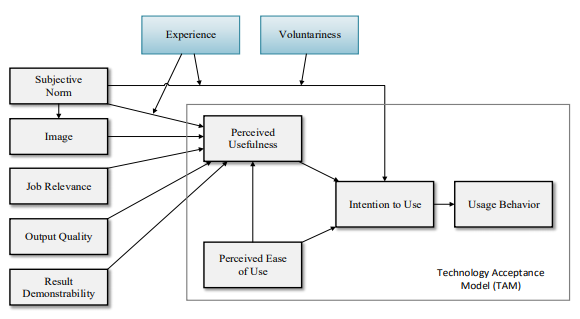
\includegraphics[width=\linewidth,height=\textheight,keepaspectratio]{Resources/TAM.png}
\caption{Technology Acceptance Modell}
\end{center}
\end{figure}




\chapter{Fokusgruppe}

In dieser Fokusgruppe wurde untersucht, wie Datenbrillen von Handwerkern aufgenommen werden und ob diese sich Szenarien vorstellen können, in welchen der Einsatz von Datenbrillen in ihrem Arbeitsumfeld hilfreich ist. Die Ursprüngliche Idee war dabei, dass Datenbrillen zur Unterstützung von Handwerkern eingesetzt werden, beispielsweise in Fernwartungsszenarien, wenn eine Person sehen möchte, was eine andere Person sieht, sich diese aber nicht am selben Ort befinden. Dann kann das Bild von der Brille des einen, zum Monitor des anderen übertragen werden. \\
Im Folgenden werden dazu die Rahmenbedingungen und die Intention, die Durchführung, sowie die Auswertung der geäußerten Ideen beschrieben. Dabei kristallisierten sich zwei Anwendungsbereiche für AR heraus, die genauer beleuchtet werden, da sie zum weiteren Verlauf dieser Forschung beitragen.

\section{Rahmen}

Um ein generelles Bild der Akzeptanz von Augmented Reality im Handwerk zu prüfen, wurde eine Fokusgruppe dazu in der Handwerkskammer München organisiert. Dazu wurden ca. 20 Handwerker aus verschiedenen handwerklichen Branchen eingeladen, um über das Thema zu diskutieren. Anfangs hielt der Moderator einen Vortrag über Augmented Reality allgemein, um den Teilnehmern die Technologie näher zu bringen. Anschließend standen verschiedene Datenbrillen, wie zum Beispiel Google Glass und die Microsoft HoloLens, zur Verfügung, welche von den Teilnehmern ausprobiert werden konnten. Die Forschungsfragen für den Workshop waren: "Was denken Handwerker über Augmented Reality, speziell Datenbrillen?" und "Können sich Handwerker Szenarien vorstellen, für welche der Einsatz von Datenbrillen für sie sinnvoll wäre?". Diese gab der Moderator den Testpersonen mit für das Testen der Brillen.

\section{Testen der Brillen}

Für jede Brille wurde eine eigene Station aufgebaut. Das Augenmerk dieser Arbeit liegt auf der Microsoft HoloLens, da dieses die am weitesten fortgeschrittene Technologie ist. Es handelt sich dabei um eine große Brille, welche mit Kameras, die ihre Umgebung filmt, sowie Mikrofon und Lautsprechern ausgestattet ist. Sie erlaubt es im Sichtfeld des Nutzers Hologramme anzuzeigen und mit diesen zu interagieren. Dieser sieht dabei die "reale Welt", welche durch die Hologramme erweitert wird. In der Fachliteratur wird dies als \textbf{Augmented Reality} oder \textbf{Mixed Reality} bezeichnet, da es reale und virtuelle Welt verschmilzt.

Das Szenario, welches mit der HoloLens nachgespielt wurde, orientierte sich an der oben genannten ursprünglichen Idee. Dies wurde mit der Applikation Skype für HoloLens und PC nachgestellt. Die Skype Applikation für HoloLens ermöglicht es dem Nutzer mit anderen über das Internet zu telefonieren. Der Nutzer sieht dabei die Webcamübertragung seines Gesprächspartners in einem Fenster-Hologramm, welches er in seiner Umgebung positionieren kann und hört diesen über die Lautsprecher der Brille. Der Nutzer am Computer sieht einen Livestream der Aufnahmen der HoloLens. Er sieht also auch Hologramme, die dieser im Raum positioniert. Beide Kommunikationspartner können mit dem Livestream und dadurch miteinander interagieren. Sie können Pfeile einzeichnen, oder Bilder in der Umgebung des HoloLensträgers platzieren. 

So ist es beispielsweise für den Brillenträger möglich dem Computernutzer ein Problem zu zeigen. Dieser kann ihn aus der Ferne beim Lösen assistieren, was in einem Laien-Experten Szenario hilfreich sein kann. Der Computernutzer erhält so einen guten Einblick in das Problem und direktes Feedback zu den Aktionen des Brillenträgers und seinen Anweisungen. Dadurch können sie sich besser abstimmen.

\section{Diskussionsrunde}

Die Diskussionsrunde wurde an einer langen Tafel abgehalten. Der Moderator stellte noch einige Applikationen und Anwendungsmöglichkeiten von Augmented Reality vor, um die Fantasie der Teilnehmer anzuregen. Danach stellte er richtungsweisende Fragen, was die Diskussion anregte. Dabei kristallisierten sich schnell zwei gefragte Themenbereiche heraus: Augmented Reality als Assistent für den Handwerker zu nutzen, der ihn bei der Ausführung seiner Arbeit unterstützt und es als visuelles Tool für das Kundengespräch zu nutzen. Die meisten Ideen drehten sich um diese Anwendungsmöglichkeiten. Zusätzlich wurde aber auch Kritik an der Microsoft HoloLens geäußert, warum sie eventuell nicht genutzt werden kann.

\subsection{Kritik an dem Einsatz von Augmented Reality und der Microsoft HoloLens}

Es wurden die hohen Anschaffungskosten kritisiert, die mit dem kauf der Microsoft HoloLens einhergehen. Diese kostet momentan ca. 3000\EURdig, was ein großer Aufwand für einen kleinen Handwerksbetrieb wäre. Dazu braucht der Handwerker auch die richtige Software, welche noch auf seine Bedürfnisse zugeschnitten werden muss. Da Teilnehmer äußerten hierzu Bedenken, dass der Kosten/Nutzen Faktor für sie nicht Interessant sein könnte.

Für das Beispiel mit Skype wurden die Bedenken geäußert, dass man dafür eine ständige, stabile Internetverbindung benötigt. Diese ist oft auf einer Baustelle oder einer großen Produktionshalle nicht gegeben. Dadurch könnten Fernwartungsapplikationen nicht verwendet werden.

Ein großer Kritikpunkt ist die Einsatzfähigkeit der HoloLens auf einer Baustelle. Dieses Umfeld ist hart, schmutzig, staubig und oft ungemütlich. Man findet schwer einen sicheren Platz zum abstellen der Brille. Bei jedem hinlegen läuft man Gefahr diese zu zerkratzen oder anderweitig zu beschädigen. Noch dazu hält sie wahrscheinlich keinen harten Stößen stand, falls sie herunterfallen sollte. Der Staub auf Baustellen kann sich negativ auf die Funktionalität der Kameras und die Darstellung der Hologramme auswirken. Gegebenenfalls erkennt die Brille dadurch die Gestensteuerung nicht mehr. Zusätzlich ist die Microsoft HoloLens ein eher unhandliches, globiges Gerät, welches man auf dem Kopf trägt. Das beeinflusst die Komfortabilität der Nutzung der Brille, vor allem bei längerem Gebrauch.

\subsection{AR als Assistent für den Handwerker}

Oft wurde von den Handwerkern der Wert einer Funktion zum automatischen Erfassen des Raumes hervorgehoben. Der initiale Prozess zum Abmessen der Wandlängen, Winkel, Einbuchtungen und sonstigem nimmt einiges an Zeit in Anspruch. Gleichzeitig handelt es sich dabei um einen wichtig Schritt, der den Grundstein für das weitere Vorgehen legt. Jeder Handwerker, sei es Fliesenleger, Maurer oder Installateur benötigt diese Daten für die Planung. Mit Augmented Reality kann es möglich sein, dies automatisch zu erfassen. Die Microsoft HoloLens beispielsweise besitzt ein integriertes \textbf{spacial mapping}, mithilfe dessen sich die Brille ein Verständnis der Umgebung verschafft. Diese Funktionalität könnte dafür genutzt werden eine solche Applikation zu integrieren. 

Nach dem erfassen des Raumes ist es für Handwerker interessant verschiedene Objekte, wie zum Beispiel Fliesen, Lampen, Fenster, Waschbecken oder ähnliches virtuell im Raum platzieren zu können. Das erleichtert die Planung, da man bereits in diesem Schritt festlegen kann, wie das Endergebnis aussieht und dadurch abschätzen kann wie viel Material benötigt wird. Das Material richtig abzuschätzen ist ein Problem, welches Handwerkern immer wieder begegnet. Zusätzlich äußerte ein Installateur die Idee, dass die Brille Verstöße gegen DIN Normen, wie beispielsweise die Höhe von Treppenstufen oder Toiletten direkt anzeigt und somit den Raum für Fehler minimiert. 

Die Datenbrille kann so also als Planungswerkzeug für den Handwerker verwendet werden. Dadurch hat er den Plan direkt vor Augen und kann ihn gegebenenfalls mit anderen Handwerkern teilen. Dies ist besonders interessant, wenn beispielsweise ein Handwerker das Kundengespräch leitet und den entstandenen Plan mit seinen Mitarbeitern teilen möchte. So kann sichergestellt werden, dass alle auf das gleiche Endergebnis hinarbeiten. Traditionell, äußerten einige Teilnehmer der Fokusgruppe, wird das oft über Telefonate abgestimmt. Dabei kommt es leicht zu Missverständnissen und somit zu Fehlern bei der Umsetzung. Eine visuelle Darstellung würde das Telefonat unterstützen und ein verständlicheres Bild zeichnen.

\subsection{AR als Assistent für das Kundengespräch}

Ein großes Problem aller Handwerker stellt das Kundengespräch dar. Sie kritisieren, dass Kunden kaum Vorstellungskraft haben. Der Handwerker kann sich das Ergebnis seiner Arbeit in einem unfertigen Raum leichter vorstellen, als der Kunde, welcher meist Laie auf dem Gebiet ist. Eine visuelle Darstellung des Plans durch Hologramme kann von diesen leichter verstanden werden, als beispielsweise ein technischer Bauplan. 

Diese visuelle Darstellung unterstützt auch beim Austausch mit dem Kunden. Dieser kann direkt sehen, wie der Handwerker seine Wünsche verstanden hat und so leichter Änderungen vorschlagen. Dadurch lassen sich Änderungswünsche, welche im späteren Verlauf der Arbeit beim Kunden auftreten könnten minimieren. Generell kann dadurch die Ambiguität in Kundengesprächen verringert werden, was eine höhere Planungssicherheit gewährleistet. 

Auch der Handwerker kann dem Kunden damit seine Vorschläge besser vor Augen führen. Die Handwerker merkten an, dass der Kunde sich oft nichts unter den Vorschlägen des Experten vorstellen kann. So werden diese ihm direkt visuell vorgeführt. Das erhöht gleichzeitig das Vertrauen in den Handwerker, da bereits beim Betrachten des Plans deutlich wird, dass DIN Normen eingehalten wurden und riskante Designs ersichtlich sind. 

Außerdem unterstützt es auch bei dem Vertragsschluss. Alle umzusetzenden Aspekte sind visuell erfassbar und dadurch digital dokumentiert. Damit lassen sich diese sehr gut im Vertrag festhalten. Es ist also für den Kunden sichergestellt, dass der Handwerker genau nach Plan vorgeht. Für den Handwerker hingegen lassen sich so Änderungen, welche vom Kunden nach der eigentlichen Vertragsschließung gefordert werden gut abgrenzen und als zusätzliche Leistungen abrechnen. 

\section{Fazit}

Ein AR Raumplaner hat, wie durch die Fokusgruppe deutlich geworden, einige Anwendungsszenarien und wird von Handwerkern gewünscht. Generell waren die Handwerker von der Technologie Augmented Reality sehr begeistert, was sich an den vielen eingebrachten Ideen zeigt. Der allgemeine Konsensus zeigt dabei auch in eine deutliche Richtung. Die ursprüngliche Idee zur Unterstützung in Fernwartungsszenarien fand nicht so viel Anklang. Handwerker interessieren sich eher für Unterstützung durch AR bei Tätigkeiten wie Maße nehmen und Planen. Auch eine visuelle Hilfe bei Kundengesprächen stellt sich als durchaus benötigt heraus. 

Allerdings wird es noch dauern, bis die Technologie ausgereift genug ist, um den Genauigkeitsansprüchen zu genügen. Die Geräte müssten für den Bau auch robuster designt und gebaut werden, um den harten Bedingungen zu trotzen. 

Zusammenfassen lässt sich jedoch sagen, dass die Datenbrillen von den Handwerkern gut akzeptiert wurden und diese Potential für die Zukunft dieser im Handwerk sehen. \\
Um diesen Ansätzen weiter nachzugehen muss tiefer in die Materie eingestiegen werden. Der Beruf eines Handwerkers muss aus der Nähe untersucht werden, um herauszufinden, wo man mit einer Applikation unterstützen kann, und ob man diese in den Arbeitsalltag eines Handwerkers integrieren kann. 

Der Beruf des Fliesenlegers würde dabei einige Aspekte abdecken. Ein Raum muss ausgemessen und darin Objekte - Fliesen - verlegt werden. Das lässt sich für Microsoft HoloLens gut umsetzen. Daher wird im nächsten Kapitel eine Ethnographie zum Beruf des Fliesenlegers angefertigt, mit dem Ziel definitive Ansatzpunkte für eine Applikation zur Unterstützung von Handwerkern, im speziellen Fliesenleger, zu erstellen.



% Optimierung für Literaturverzeichnis
\setcounter{biburllcpenalty}{8000}
\setcounter{biburlucpenalty}{8000}

% Literaturverzeichnis generieren.
% Inhalt erscheint, sobald Einträge in der Bib hinterlegt sind!
\cleardoublepage
\addcontentsline{toc}{chapter}{Literaturverzeichnis}
\printbibliography[title={Literaturverzeichnis}]

% Abbildungsverzeichnis generieren.
\cleardoublepage
\addcontentsline{toc}{chapter}{\listfigurename}
\listoffigures


% Tabellenverzeichnis generieren.
%\cleardoublepage
%\addcontentsline{toc}{chapter}{\listtablename}
%\listoftables

% Listingverzeichnis generieren.
\cleardoublepage
\renewcommand{\lstlistlistingname}{Listingverzeichnis}
\addcontentsline{toc}{chapter}{\lstlistlistingname}
\lstlistoflistings

%
%% Anhang einfügen.
%\cleardoublepage
%\begin{appendix}
\chapter{<Kapitel im Anhang>}
Hier kommt der Anhang rein ...
\end{appendix}

% Glossar generieren
\glsaddall
\printglossaries

\end{document}
